%% Part of Stellarium User Guide
%% Status: 2015-12-30 Some parts collected from wiki.
%%         2016-04-05 GZ changed to have 1 chapter per plugin for a better structure. This file may be split up later. 
%% TODO: All plugins! And give a better structure than just by alphabet.

\chapter{Built-in Plugins}
Since version 0.10.3, Stellarium's packages include a number of plug-ins.

\section{Angle Measure Plugin}
\label{sec:plugins:AngleMeasure}

%\url{http://porpoisehead.net/images/plugin-angle-measure.jpg}

The Angle Measure plugin is a small tool which is used to measure the
angular distance between two points on the sky. 

\small{*goes misty eyed*\\ 
I recall measuring the size of the Cassini Division when I was a student.
It was not the high academic glamor one might expect... It was cloudy...
It was rainy... The observatory lab had some old scopes set up at one
end, pointing at a \emph{photograph} of Saturn at the other end of the
lab. We measured. We calculated. We wished we were in Hawaii. A picture
is worth a thousand words.}

\subsection{Using the plugin}
\label{sec:plugins:AngleMeasure:using}

\begin{enumerate}
\item
  Enable the tool by clicking the tool-bar button, or by pressing
  \textbf{control-A}. A message will appear at the bottom of the screen
  to tell you that the tool is active.
\item
  Drag a line from the first point to the second point using the left
  mouse button
\item
  To clear the measurement, click the right mouse button
\item
  To deactivate the angle measure tool, press the tool-bar button again,
  or press \textbf{control-A} on the keyboard.
\end{enumerate}

\newpage

\section{Bright Novae Plugin}
\label{sec:plugins:BrightNovae}

The Bright Novae plugin provides visualization of some bright novae in
the Milky Way galaxy (Fig.~\ref{fig:NovaCygni1975}).

%Example (\href{http://en.wikipedia.org/wiki/V1500_Cygni}{\textbf{Nova
%Cygni 1975}}, also known as \textbf{V1500 Cyg}):

\begin{figure}[h]
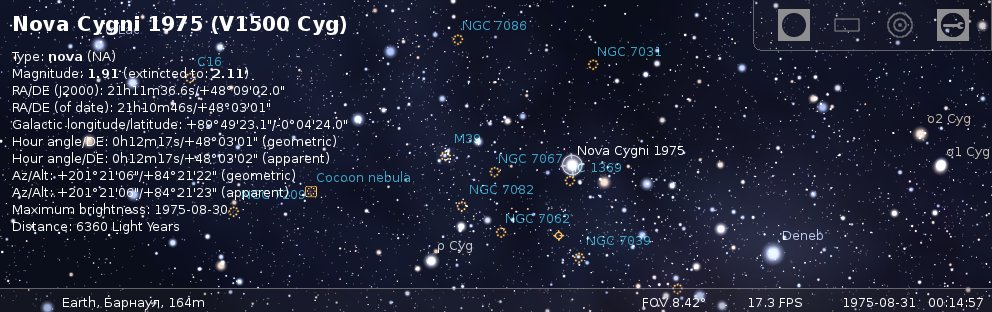
\includegraphics[width=\textwidth]{NovaCygni1975wiki.jpg}
\label{fig:NovaCygni1975}
\caption{Nova Cygni 1975 (also known as \textbf{V1500 Cyg})}
\end{figure}

\subsection{Using the Bright Novae plugin}
\label{sec:plugins:BrighrNovae:using}

\begin{enumerate}
\item Enable the tool by clicking the tool-bar button ``Load at startup''
\item Set date and time (30 August 1975 year for \emph{Nova Cygni 1975} as example\footnote{\url{http://en.wikipedia.org/wiki/V1500_Cygni}})
\end{enumerate}

\subsection{Section \big[Novae\big] in config.ini file}
\label{sec:plugins:BrightNovae:config}

You can edit \file{config.ini} file by yourself for changes of the
settings for the Bright Novae plugin -- just make it carefully!

\begin{longtabu} to \textwidth {l|l|X}\toprule
\emph{ID}            & \emph{Type} & \emph{Description}\\\midrule
last\_update            & string & Date and time of last update\\\midrule
update\_frequency\_days & int    & Frequency of updates, in days\\\midrule
updates\_enable         & bool   & Enable updates of bright novae catalog from Internet \\\midrule
url                     & string & URL of bright novae catalog \\\bottomrule
\end{longtabu}

\subsection{Format of bright novae catalog}
\label{sec:plugins:BrightNovae:format}

To add a new nova, open a new line after line 5 and paste the following, note commas and brackets, they are important:

\begin{configfile}
"Nova designation":
{
    "name": "name of nova",
    "type": "type of nova",
    "maxMagnitude": value of maximal visual magnitude,
    "minMagnitude": value of minimal visual magnitude,
    "peakJD": JD for maximal visual magnitude,
    "m2": Time to decline by 2mag from maximum (in days),
    "m3": Time to decline by 3mag from maximum (in days),
    "m6": Time to decline by 6mag from maximum (in days),
    "m9": Time to decline by 9mag from maximum (in days),
    "distance": value of distance between nova and 
                Earth (in thousands of Light Years),
    "RA": "Right ascension (J2000)",
    "Dec": "Declination (J2000)"
},
\end{configfile}

\noindent For example, the record for \textbf{Nova Cygni 1975} (\textbf{V1500 Cyg}) looks like:
\begin{configfile}
"V1500 Cyg":
{
    "name": "Nova Cygni 1975",
    "type": "NA",
    "maxMagnitude": 1.69,
    "minMagnitude": 21,
    "peakJD": 2442655,
    "m2": 2,
    "m3": 4,
    "m6": 32,
    "m9": 263
    "distance": 6.36,
    "RA": "21h11m36.6s",
    "Dec": "48d09m02s"
},
\end{configfile}

\subsection{Light curves}
\label{sec:plugins:BrightNovae:lightcurves}

This plugin uses a very simple model for calculation of light curves for
novae stars. This model is based on time for decay by $N$
magnitudes from the maximum value, where $N$ is 2, 3, 6 and 9. If a
nova has no values for decay of magnitude then this plugin will use
generalized values for it.

\newpage

\section{Compass Marks Plugin}
\label{sec:plugins:CompassMarks}

%\url{http://porpoisehead.net/images/plugin-compass-marks.jpg}

Stellarium helps the user get their bearings using the cardinal point
feature - the North, South, East and West markers on the horizon.
Compass Marks takes this idea and extends it to add markings every few
degrees along the horizon, and includes compass bearing values in
degrees.

\subsection{Using the plugin}
\label{sec:plugins:CompassMarks:using}

There is a tool bar button for toggling the compass markings, or you can
press \key{control-C}.

Note that when you first enable compass marks, the cardinal points will
be turned off. You can have both active at once, but there is a small
bug which means you have to press \key{Q} \emph{two times} to
re-enable cardinal points after enabling the compass markings.

\newpage

\section{Equation of Time Plugin}
\label{sec:plugins:EquationOfTime}
The Equation of Time plugin shows the solution of the equation of time (Fig.~\ref{fig:EqOfTime}).

\begin{figure}[h]
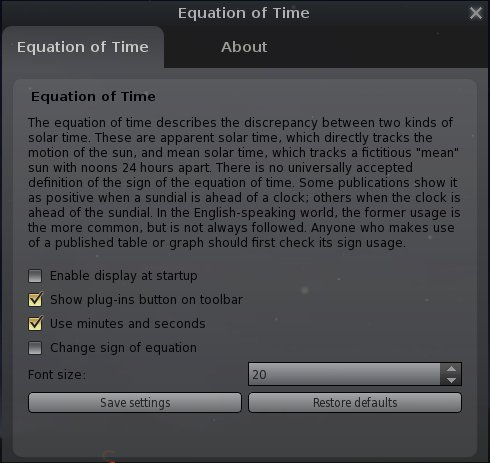
\includegraphics[width=\textwidth]{EquationOfTime-plugin.jpg}
\label{fig:EqOfTime}
\caption{Interface of Equation of Time plugin}
\end{figure}

The equation of time describes the discrepancy between two kinds of solar time. These are apparent solar time, which directly tracks the motion of the sun, and mean solar time, which tracks a fictitious ``mean'' sun with noons 24 hours apart. There is no universally accepted definition of the sign of the equation of time. Some publications show it as positive when a sundial is ahead of a clock; others when the clock is ahead of the sundial. In the English-speaking world, the former usage is the more common, but is not always followed. Anyone who makes use of a published table or graph should first check its sign usage.

\subsection{Using the Equation of Time plugin}
\label{sec:plugins:EquationOfTime:using}

\begin{enumerate}
\item Enable the tool by clicking the tool-bar button ``Load at startup''.
\item Click on the Equation of Time button on the bottom toolbar for displaying solution for equation of time on top of the screen.
\end{enumerate}

\subsection{Section \big[EquationOfTime\big] in config.ini file}
\label{sec:plugins:EquationOfTime:config}

You can edit \file{config.ini} file by yourself for changes of the
settings for the Equation of Time plugin -- just make it carefully!

\begin{longtabu} to \textwidth {l|l|X}\toprule
\emph{ID}            & \emph{Type} & \emph{Description}\\\midrule
enable\_at\_startup  & bool & Display solution of the equation of time at startup of the planetarium\\\midrule
flag\_use\_ms\_format & bool & Set format for the displayed solution - minutes and seconds and decimal minutes\\\midrule
flag\_use\_inverted\_value & bool & Change sign of the equation of time \\\midrule
flag\_show\_button & bool & Enable displaying plugin button on the bottom toolbar\\\midrule
text\_color & R,G,B & Color of font for the displayed solution of the equation of time\\\midrule
font\_size & int & Font size for the displayed solution of the equation of time \\\bottomrule
\end{longtabu}

\newpage

\section{Exoplanets Plugin}
\label{sec:plugins:Exoplanets}
This plugin plots the position of stars with exoplanets. Exoplanets data is derived from ``The Extrasolar Planets Encyclopaedia''\footnote{\url{http://exoplanet.eu/}}. List of potential habitable exoplanets and data about them were taken from ``The Habitable Exoplanets Catalog''\footnote{\url{http://phl.upr.edu/projects/habitable-exoplanets-catalog}} by Planetary Habitability Laboratory\footnote{\url{http://phl.upr.edu/home}}.

\begin{figure}[h]
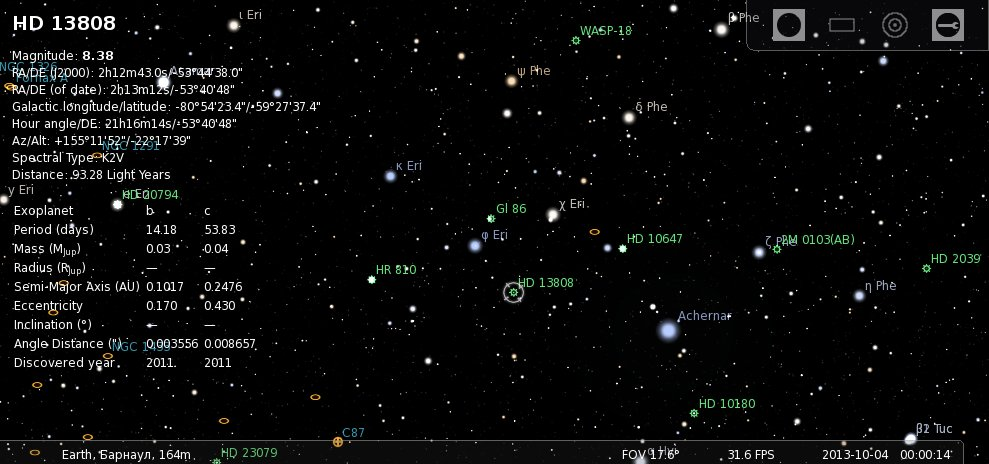
\includegraphics[width=\textwidth]{exoplanets.jpg}
\label{fig:Exoplanets}
\caption{Planetary system HD 13808}
\end{figure}

\subsection{Potential habitable exoplanets}
\label{sec:plugins:Exoplanets:habitable}
This plugin can display potential habitable exoplanets (orange marker) and some information about those planets.

\paragraph{Planetary Class}
Planet classification from host star spectral type (F, G, K, M), habitable zone (hot, warm, cold) and size (miniterran, subterran, terran, superterran, jovian, neptunian) (Earth = G-Warm Terran).

\paragraph{Equilibrium Temperature}
The planetary equilibrium temperature\footnote{\url{http://lasp.colorado.edu/~bagenal/3720/CLASS6/6EquilibriumTemp.html}} is a theoretical temperature in (\degree C) that the planet would be at when considered simply as if it were a black body being heated only by its parent star (assuming a 0.3 bond albedo). As example the planetary equilibrium temperature of Earth is -18.15\degree C (255 K).

\paragraph{Earth Similarity Index (ESI)}
Similarity to Earth\footnote{\url{http://phl.upr.edu/projects/earth-similarity-index-esi}} on a scale from 0 to 1, with 1 being the most Earth-like. ESI depends on the planet's radius, density, escape velocity, and surface temperature.

\subsection{Proper names}
\label{sec:plugins:Exoplanets:ProperNames}
In December 2015, the International Astronomical Union (IAU) has officially approved names for several exoplanets after a public vote.
\begin{itemize}
\item \textbf{Veritate}* (14 And) -- From the latin Veritas, truth. The ablative form means \textit{where there is truth}\footnote{The original name proposed, Veritas, is that of an asteroid important for the study of the solar system.}.
\item \textbf{Spe}* (14 And b) -- From the latin Spes, hope. The ablative form means \textit{where there is hope}.
\item \textbf{Musica} (18 Del) -- Musica is Latin for \textit{music}.
\item \textbf{Arion} (18 Del b) -- Arion was a genius of poetry and music in ancient Greece. According to legend, his life was saved at sea by dolphins after attracting their attention by the playing of his kithara.
\item \textbf{Fafnir} (42 Dra) -- Fafnir was a Norse mythological dwarf who turned into a dragon.
\item \textbf{Orbitar} (42 Dra b) -- Orbitar is a contrived word paying homage to the space launch and orbital operations of NASA.
\item \textbf{Chalawan} (47 UMa) -- Chalawan is a mythological crocodile king from a Thai folktale.
\item \textbf{Taphao Thong} (47 UMa b) -- Taphao Thong is one of two sisters associated with the Thai folk tale of Chalawan.
\item \textbf{Taphao Kaew} (47 UMa c) -- Taphao Kae is one of two sisters associated with the Thai folk tale of Chalawan.
\item \textbf{Helvetios} (51 Peg) -- Helvetios is Celtic for the \textit{Helvetian} and refers to the Celtic tribe that lived in Switzerland during antiquity.
\item \textbf{Dimidium} (51 Peg b) -- Dimidium is Latin for \textit{half}, referring to the planet's mass of at least half the mass of Jupiter.
\item \textbf{Copernicus} (55 Cnc) -- Nicolaus Copernicus or Mikolaj Kopernik (1473-1543) was a Polish astronomer who proposed the heliocentric model of the solar system in his book ``De revolutionibus orbium coelestium''.
\item \textbf{Galileo} (55 Cnc b) -- Galileo Galilei (1564-1642) was an Italian astronomer and physicist often called the \textit{father of observational astronomy} and the \textit{father of modern physics}. Using a telescope, he discovered the four largest satellites of Jupiter, and the reported the first telescopic observations of the phases of Venus, among other discoveries.
\item \textbf{Brahe} (55 Cnc c) -- Tycho Brahe (1546-1601) was a Danish astronomer and nobleman who recorded accurate astronomical observations of the stars and planets. These observations were critical to Kepler's formulation of his three laws of planetary motion.
\item \textbf{Lipperhey}* (55 Cnc d) -- Hans Lipperhey (1570-1619) was a German-Dutch lens grinder and spectacle maker who is often attributed with the invention of the refracting telescope in 1608\footnote{The original spelling of Lippershey was corrected to Lipperhey on 15.01.2016. The commonly seen spelling Lippershey (with an s) results in fact from a typographical error dating back from 1831, thus should be avoided.}.
\item \textbf{Janssen} (55 Cnc e) -- Jacharias Janssen (1580s-1630s) was a Dutch spectacle maker who is often attributed with invention of the microscope, and more controversially with the invention of the telescope.
\item \textbf{Harriot} (55 Cnc f) -- Thomas Harriot (ca. 1560-1621) was an English astronomer, mathematician, ethnographer, and translator, who is attributed with the first drawing of the Moon through telescopic observations.
\item \textbf{Amateru}* ($\epsilon$ Tau b) -- \textit{Amateru} is a common Japanese appellation for shrines when they enshrine Amaterasu, the Shinto goddess of the Sun, born from the left eye of the god Izanagi\footnote{The name originally proposed, Amaterasu, is already used for an asteroid.}.
\item \textbf{Hypatia} ($\iota$ Dra b) -- Hypatia was a famous Greek astronomer, mathematician, and philosopher. She was head of the Neo-Platonic school at Alexandria in the early 5th century, until murdered by a Christian mob in 415.
\item \textbf{Ran}* ($\epsilon$ Eri) -- Ran is the Norse goddess of the sea, who stirs up the waves and captures sailors with her net.
\item \textbf{AEgir}* ($\epsilon$ Eri b) -- AEgir is Ran's husband, the personified god of the ocean. \textit{AEgir} and \textit{Ran} both represent the \textit{Jotuns} who reign in the outer Universe; together they had nine daughters\footnote{Note the typographical difference between AEgir and Aegir, the Norwegian transliteration. The same name, with the spelling Aegir, has been attributed to one of Saturn's satellites, discovered in 2004.}.
\item \textbf{Tadmor}* ($\gamma$ Cep b) -- Ancient Semitic name and modern Arabic name for the city of Palmyra, a UNESCO World Heritage Site.
\item \textbf{Dagon} ($\alpha$ PsA b) -- Dagon was a Semitic deity, often represented as half-man, half-fish.
\item \textbf{Tonatiuh} (HD 104985) -- Tonatiuh was the Aztec god of the Sun.
\item \textbf{Meztli} (HD 104985 b) -- Meztli was the Aztec goddess of the Moon.
\item \textbf{Ogma}* (HD 149026) -- Ogma was a deity of eloquence, writing, and great physical strength in the Celtic mythologies of Ireland and Scotland, and may be related to the Gallo-Roman deity \textit{Ogmios}\footnote{Ogmios is a name already attributed to an asteroid.}.
\item \textbf{Smertrios} (HD 149026 b) -- Smertrios was a Gallic deity of war.
\item \textbf{Intercrus} (HD 81688) -- Intercrus means \textit{between the legs} in Latin style, referring to the star's position in the constellation Ursa Major.
\item \textbf{Arkas} (HD 81688 b) -- Arkas was the son of Callisto (Ursa Major) in Greek mythology.
\item \textbf{Cervantes} ($\mu$ Ara) -- Miguel de Cervantes Saavedra (1547-1616) was a famous Spanish writer and author of ``El Ingenioso Hidalgo Don Quixote de la Mancha''.
\item \textbf{Quijote} ($\mu$ Ara b) -- Lead fictional character from Cervantes's ``El Ingenioso Hidalgo Don Quixote de la Mancha''.
\item Dulcinea ($\mu$ Ara c) — Fictional character and love interest of Don Quijote (or Quixote) in Cervantes's ``El Ingenioso Hidalgo Don Quixote de la Mancha''.
\item \textbf{Rocinante} ($\mu$ Ara d) -- Fictional horse of Don Quijote in Cervantes's ``El Ingenioso Hidalgo Don Quixote de la Mancha''.
\item \textbf{Sancho} ($\mu$ Ara e) -- Fictional squire of Don Quijote in Cervantes's ``El Ingenioso Hidalgo Don Quixote de la Mancha''.
\item \textbf{Thestias}* ($\beta$ Gem b) -- Thestias is the patronym of Leda and her sister Althaea, the daughters of Thestius. Leda was a Greek queen, mother of Pollux and of his twin Castor, and of Helen and Clytemnestra\footnote{The original proposed name Leda is already attributed to an asteroid and to one of Jupiter's satellites. The name Althaea is also attributed to an asteroid.}.
\item \textbf{Lich} (PSR B1257+12) -- Lich is a fictional undead creature known for controlling other undead creatures with magic.
\item \textbf{Draugr} (PSR B1257+12 b) -- Draugr refers to undead creatures in Norse mythology.
\item \textbf{Poltergeist} (PSR B1257+12 c) -- Poltergeist is a name for supernatural beings that create physical disturbances, from German for noisy ghost.
\item \textbf{Phobetor} (PSR B1257+12 d) -- Phobetor is a Greek mythological deity of nightmares, the son of Nyx, the primordial deity of night.
\item \textbf{Titawin} ($\upsilon$ And) -- Titawin (also known as Medina of Tetouan) is a settlement in northern Morocco and UNESCO World Heritage Site. Historically it was an important point of contact between two civilizations (Spanish and Arab) and two continents (Europe and Africa) after the $8^{th}$ century.
\item \textbf{Saffar} ($\upsilon$ And b) -- Saffar is named for Abu al-Qasim Ahmed Ibn-Abd Allah Ibn-Omar al Ghafiqi Ibn-al-Saffar, who taught arithmetic, geometry, and astronomy in 11th century Cordova in Andalusia (modern Spain), and wrote an influential treatise on the uses of the astrolabe.
\item \textbf{Samh} ($\upsilon$ And c) -- Samh is named for Abu al-Qasim 'Asbagh ibn Muhammad ibn al-Samh al-Mahri (or Ibn al-Samh), a noted 11th century astronomer and mathematician in the school of al Majriti in Cordova (Andalusia, now modern Spain).
\item \textbf{Majriti} ($\upsilon$ And d) -- Majriti is named for Abu al-Qasim al-Qurtubi al-Majriti, a notable mathematician, astronomer, scholar, and teacher in $10^{th}$ century and early $11^{th}$ century Andalusia (modern Spain).
\item \textbf{Libertas}* ($\xi$ Aql) -- Libertas is Latin for liberty. Liberty refers to social and political freedoms, and a reminder that there are people deprived of liberty in the world even today. The constellation Aquila represents an eagle -- a popular symbol of liberty.
\item \textbf{Fortitudo}* ($\xi$ Aql b) -- Fortitudo is Latin for fortitude. Fortitude means emotional and mental strength in the face of adversity, as embodied by the eagle (represented by the constellation Aquila).
\end{itemize}

All names with asterix mark (*) are modified based on the original proposals, to be consistent with the IAU rules.

\subsection{Using the Exoplanets plugin}
\label{sec:plugins:Exoplanets:using}

\begin{enumerate}
\item Enable the tool by clicking the tool-bar button ``Load at startup''.
\item Find the stars with exoplanets by their designation (24 Sex as example).
\end{enumerate}

\subsection{Section \big[Exoplanets\big] in config.ini file}
\label{sec:plugins:Exoplanets:config}

You can edit \file{config.ini} file by yourself for changes of the
settings for the Exoplanets plugin -- just make it carefully!

\begin{longtabu} to \textwidth {l|l|X}\toprule
\emph{ID}            & \emph{Type} & \emph{Description}\\\midrule
last\_update  & string & Date and time of last update \\\midrule
update\_frequency\_hours  & int & Frequency of updates, in hours \\\midrule
updates\_enable  & bool & Enable updates of exoplanets catalog from Internet \\\midrule
url  & string & URL of exoplanets catalog \\\midrule
flag\_show\_exoplanets\_button  & bool & Enable showing button of exoplanets on bottom bar \\\midrule
distribution\_enabled  & bool & Enable distribution mode of display \\\midrule
timeline\_enabled  & bool & Enable timeline mode of display \\\midrule
habitable\_enabled  & bool & Enable habitable mode of display \\\midrule
enable\_at\_startup  & bool & Enable displaying exoplanets at startup of the plugin \\\midrule
exoplanet\_marker\_color & R,G,B & Color for marker of star with planetary system \\\midrule
habitable\_exoplanet\_marker\_color  & R,G,B & Color for marker of star with planetary system with potential habitable exoplanets
 \\\bottomrule
\end{longtabu}

\subsection{Format of exoplanets catalog}
\label{sec:plugins:Exoplanets:format}

To add a new exoplanet system, open a new line after line 5 and paste the following, note commas and brackets, they are important:

\begin{configfile}
"Star designation":
{
	"exoplanets":
	[
	{
		"mass": mass of exoplanet (M jup),
		"radius": radius of exoplanet (R jup),
		"period": period of exoplanet (days),
		"semiAxis": semi-major axis (AU),
		"eccentricity": orbit's eccentricity,
		"inclination": orbit's inclination (degree),
		"angleDistance": angle distance from star 
		                 (arcseconds),
		"discovered": exoplanet discovered year,
		"hclass": "habitable class",
		"MSTemp": mean surface temperature (K),
		"ESI": Earth Similarity Index (*100),
		"planetProperName": "proper name of planet",
		"planetName": "designation of planet"
	},
	{
		"mass": mass of exoplanet (M jup),
		"radius": radius of exoplanet (R jup),
		"period": period of exoplanet (days),
		"semiAxis": semi-major axis (AU),
		"eccentricity": orbit's eccentricity,
		"inclination": orbit's inclination (degree),
		"angleDistance": angle distance from star 
		                 (arcseconds),
		"discovered": exoplanet discovered year,
		"hclass": "habitable class",
		"MSTemp": mean surface temperature (K),
		"ESI": Earth Similarity Index (*100),
		"planetProperName": "proper name of planet",
		"planetName": "designation of planet"
	}
	],
	"distance": value of distance to star (pc),
	"stype": "spectral type of star",
	"smass": value of mass of star (M sun),
	"smetal": value of metallicity of star,
	"Vmag": value of visual magnitude of star,
	"sradius": value of radius of star (R sun),
	"effectiveTemp": value of effective temperature 
	                 of star (K),
	"starProperName": "proper name of the star",
	"hasHP": boolean (has potential habitable planets),
	"RA": "Right ascension (J2000)",
	"DE": "Declination (J2000)"
},
\end{configfile}

\noindent For example, record for \textit{24 Sex} looks like:
\begin{configfile}
"24 Sex":
{
		"exoplanets":
		[
		{
			"mass": 1.99,
			"period": 452.8,
			"semiAxis": 1.333,
			"eccentricity": 0.09,
			"angleDistance": 0.017821,
			"discovered": 2010,
			"planetName": "b"
		},
		{
			"mass": 0.86,
			"period": 883.0,
			"semiAxis": 2.08,
			"eccentricity": 0.29,
			"angleDistance": 0.027807,
			"discovered": 2010,
			"planetName": "c"
		}
		],
		"distance": 74.8,
		"stype": "G5",
		"smass": 1.54,
		"smetal": -0.03,
		"Vmag": 7.38,
		"sradius": 4.9,
		"effectiveTemp": 5098,
		"RA": "10h23m28s",
		"DE": "-00d54m08s"
},
\end{configfile}

\newpage
\section{Field of View Plugin}
\label{sec:plugins:FieldOfView}
The Field of View plugin allows stepwise zooming via keyboard shortcuts like in the Cartes du Ciel\footnote{Official website of SkyChart / Cartes du Ciel planetarium -- \url{http://www.ap-i.net/skychart/en/start}} planetarium program.

\begin{figure}[h]
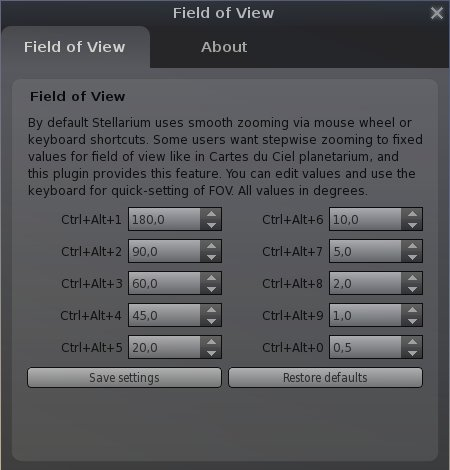
\includegraphics[width=\textwidth]{FOV-plugin.jpg}
\label{fig:FieldOfView}
\caption{Interface of Field of View plugin}
\end{figure}

By default Stellarium uses smooth zooming via mouse wheel or keyboard shortcuts. Some users want stepwise zooming to fixed values for field of view like in Cartes du Ciel planetarium, and this plugin provides this feature. You can edit values and use the keyboard for quick-setting of FOV. All values in degrees.

\subsection{Using the Field of View plugin}
\label{sec:plugins:FieldOfView:using}

\begin{enumerate}
\item Enable the tool by clicking the tool-bar button ``Load at startup''.
\item Press shortkeys for quick changes of FOV.
\end{enumerate}

\subsection{Section \big[FOV\big] in config.ini file}
\label{sec:plugins:FieldOfView:config}

You can edit \file{config.ini} file by yourself for changes of the
settings for the Field of View plugin -- just make it carefully!

\begin{longtabu} to \textwidth {l|l|X}\toprule
\emph{ID}            & \emph{Type} & \emph{Description}\\\midrule
fov\_quick\_0  & float & Value of FOV for the shortcut ``Ctrl+Alt+0'' \\\midrule
fov\_quick\_1  & float & Value of FOV for the shortcut ``Ctrl+Alt+1'' \\\midrule
fov\_quick\_2  & float & Value of FOV for the shortcut ``Ctrl+Alt+2'' \\\midrule
fov\_quick\_3  & float & Value of FOV for the shortcut ``Ctrl+Alt+3'' \\\midrule
fov\_quick\_4  & float & Value of FOV for the shortcut ``Ctrl+Alt+4'' \\\midrule
fov\_quick\_5  & float & Value of FOV for the shortcut ``Ctrl+Alt+5'' \\\midrule
fov\_quick\_6  & float & Value of FOV for the shortcut ``Ctrl+Alt+6'' \\\midrule
fov\_quick\_7  & float & Value of FOV for the shortcut ``Ctrl+Alt+7'' \\\midrule
fov\_quick\_8  & float & Value of FOV for the shortcut ``Ctrl+Alt+8'' \\\midrule
fov\_quick\_9  & float & Value of FOV for the shortcut ``Ctrl+Alt+9'' \\\bottomrule
\end{longtabu}

\newpage

\section{Historical Supernovae Plugin}
\label{sec:plugins:HistoricalSupernovae}
The Historical Supernovae plugin provides visualization of some bright historical supernovae (Fig.~\ref{fig:SN1604}) from table below\footnote{List of supernovae in default catalog.}.

\begin{longtabu} to \textwidth {l|l|l|l|X}\toprule
\emph{Supernova}            & \emph{Date of max. brightness} & \emph{Max. apparent mag.} & \emph{Type} & \emph{Name} \\\midrule
SN 185A\footnote{\url{https://en.wikipedia.org/wiki/SN_185}} & 7 December & -6.0 & Ia & \\\midrule
SN 386A & 24 April & 1.5 & II & \\\midrule
SN 1006A\footnote{\url{https://en.wikipedia.org/wiki/SN_1006}} & 29 April & -7.5 & I & \\\midrule
SN 1054A\footnote{\url{https://en.wikipedia.org/wiki/SN_1054}} & 3 July & -6.0 & II & \\\midrule
SN 1181A\footnote{\url{https://en.wikipedia.org/wiki/SN_1181}} & 4 August & -2.0 & II & \\\midrule
SN 1572A\footnote{\url{https://en.wikipedia.org/wiki/SN_1572}} & 5 November & -4.0 & I & Tycho's Supernova\\\midrule
SN 1604A\footnote{\url{https://en.wikipedia.org/wiki/SN_1604}} & 8 October & -2.0 & I & Kepler's Supernova\\\midrule
SN 1680A\footnote{\url{https://en.wikipedia.org/wiki/Cassiopeia_A}} & 15 August & 6.0 & IIb & Cassiopeia A\\\midrule
SN 1885A\footnote{\url{https://en.wikipedia.org/wiki/S_Andromedae}} & 17 August & 5.8 & IPec & S Andromedae\\\midrule
SN 1895B & 5 July & 8.0 & I & \\\midrule
SN 1920A & 17 December & 11.7 & II & \\\midrule
SN 1921C & 11 December & 11.0 & I & \\\midrule
SN 1937C & 21 August & 8.5 & Ia & \\\midrule
SN 1960F & 21 April & 11.6 & Ia & \\\midrule
SN 1960R & 19 December & 12.0 & I & \\\midrule
SN 1961H & 8 May & 11.8 & Ia & \\\midrule
SN 1962M & 26 November & 11.5 & II & \\\midrule
SN 1966J & 2 December & 11.3 & I & \\\midrule
SN 1968L & 12 July & 11.9 & IIP & \\\midrule
SN 1970G & 30 July & 11.4 & IIL & \\\midrule
SN 1971I & 29 May & 11.9 & Ia & \\\midrule
SN 1972E\footnote{\url{https://en.wikipedia.org/wiki/SN1972e}} & 8 May & 8.4 & Ia & \\\midrule
SN 1979C & 15 April & 11.6 & IIL & \\\midrule
SN 1980K & 31 October & 11.6 & IIL & \\\midrule
SN 1981B & 9 March & 12.0 & Ia & \\\midrule
SN 1983N & 17 July & 11.4 & Ib & \\\midrule
SN 1987A\footnote{\url{https://en.wikipedia.org/wiki/SN_1987A}} & 24 February & 2.9 & IIPec & \\\midrule
SN 1989B & 6 February & 11.9 & Ia & \\\midrule
SN 1991T & 26 April & 11.6 & IaPec & \\\midrule
SN 1993J\footnote{\url{https://en.wikipedia.org/wiki/SN_1993J}} & 30 March & 10.8 & IIb & \\\midrule
SN 1994D & 31 March & 11.8 & Ia & \\\midrule
SN 1998bu & 21 May & 11.9 & Ia & \\\midrule
SN 2004dj & 31 July & 11.3 & IIP & \\\midrule
SN 2011fe\footnote{\url{https://en.wikipedia.org/wiki/SN_2011fe}} & 13 September & 10.06 & Ia & \\\midrule
SN 2013aa & 13 February	& 11.9 & Ia & \\\bottomrule
\end{longtabu}

\begin{figure}[h]
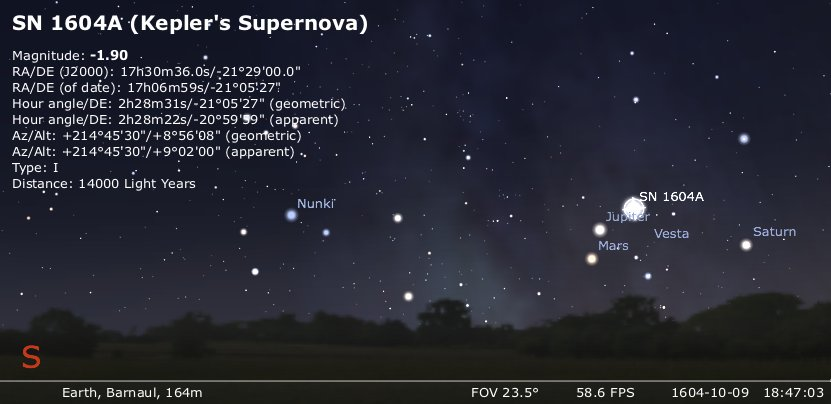
\includegraphics[width=\textwidth]{sn1604wiki.jpg}
\label{fig:SN1604}
\caption{Supernova 1604 (also known as \textbf{Kepler's Supernova}, \textbf{Kepler's Nova} or \textbf{Kepler's Star}}
\end{figure}

\subsection{Using the Historical Supernovae plugin}
\label{sec:plugins:HistoricalSupernovae:using}

\begin{enumerate}
\item Enable the tool by clicking the tool-bar button ``Load at startup''.
\item Set date and time (29 April 1006 year for \emph{SN 1006A} as example\footnotemark[16]).
\end{enumerate}

\subsection{Section \big[Supernovae\big] in config.ini file}
\label{sec:plugins:HistoricalSupernovae:config}

You can edit \file{config.ini} file by yourself for changes of the
settings for the Historical Supernovae plugin -- just make it carefully!

\begin{longtabu} to \textwidth {l|l|X}\toprule
\emph{ID}            & \emph{Type} & \emph{Description}\\\midrule
last\_update            & string & Date and time of last update\\\midrule
update\_frequency\_days & int    & Frequency of updates, in days\\\midrule
updates\_enable         & bool   & Enable updates of bright novae catalog from Internet \\\midrule
url                     & string & URL of bright novae catalog \\\bottomrule
\end{longtabu}

\subsection{Format of historical supernovae catalog}
\label{sec:plugins:HistoricalSupernovae:format}

To add a new nova, open a new line after line 5 and paste the following, note commas and brackets, they are important:

\begin{configfile}
"Supernova designation":
{
    "type": "type of supernova",
    "maxMagnitude": value of maximal visual magnitude,
    "peakJD": JD for maximal visual magnitude,
    "alpha": "Right ascension (J2000)",
    "delta": "Declination (J2000)",
    "distance": value of distance between supernova and 
                Earth (in thousands of Light Years),
    "note": "notes for supernova"
},
\end{configfile}

\noindent For example, the record for \textbf{SN 1604A} (\textbf{Kepler's Supernova}) looks like:
\begin{configfile}
"1604A":
{
    "type": "I",
    "maxMagnitude": -2,
    "peakJD": 2307190,
    "alpha": "17h30m36.00s",
    "delta": "-21d29m00.0s",
    "distance": 14,
    "note": "Kepler's Supernova"
},
\end{configfile}

\newpage
\subsection{Light curves}
\label{sec:plugins:HistoricalSupernovae:lightcurves}

In this plugin implemented simple model of light curves for different supernovae. Typical view of light curve for supernova type I you can see on Fig.~\ref{fig:SNTypeI} (bottom scale in days) and this model used for plugin.

\begin{figure}[h]
\begin{center}
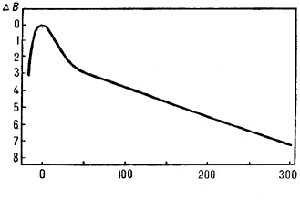
\includegraphics[width=250px]{sn_type_I.jpg}
\end{center}
\label{fig:SNTypeI}
\caption{Light Curve of Supernova Type I}
\end{figure}

For supernova type II we use typical light curve with plato, which you can see on Fig.~\ref{fig:SNTypeII} (bottom scale in days).

\begin{figure}[h]
\begin{center}
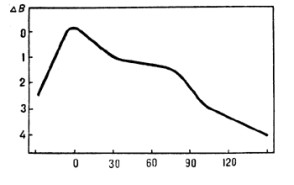
\includegraphics[width=260px]{sn_type_II.jpg}
\end{center}
\label{fig:SNTypeII}
\caption{Light Curve of Supernova Type II}
\end{figure}

On both images for light curves of maximum brightness marked as day 0.

\newpage

\section{Meteor Showers Plugin}
\label{sec:plugins:MeteorShowers}

This plugin displays meteor showers and a marker for each active and inactive radiant, showing real information about its activity\footnote{This plugin was created as project of ESA Summer of Code in Space 2013 -- \url{http://sophia.estec.esa.int/socis2013/?q=about}}.

\begin{figure}[h]
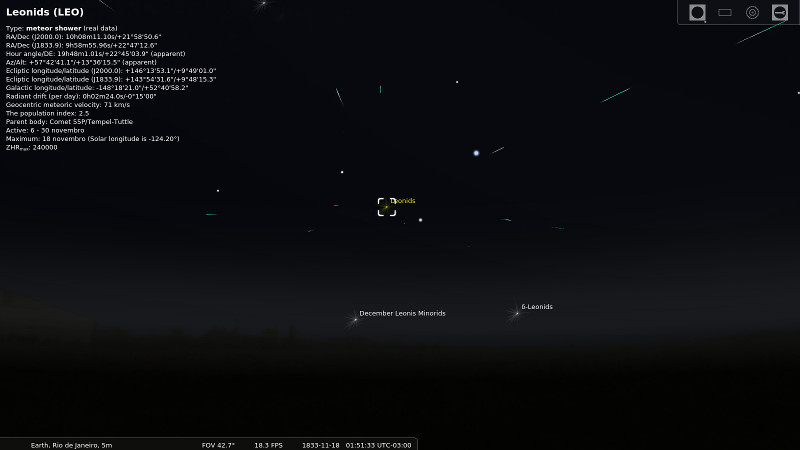
\includegraphics[width=\textwidth]{meteorshowers.jpg}
\label{fig:MeteorShowers}
\caption{Leonids 1833}
\end{figure}

Info about meteor showers you can get here:
\begin{itemize}
\item Meteor shower -- \url{https://en.wikipedia.org/wiki/Meteor_Showers}
\item International Meteor Organization -- \url{http://www.imo.net/}
\end{itemize}

\subsection{Terms}
\label{sec:plugins:MeteorShowers:terms}

\paragraph{Meteor shower}
A meteor shower is a celestial event in which a number of meteors are observed to radiate, or originate, from one point in the night sky. These meteors are caused by streams of cosmic debris called meteoroids entering Earth's atmosphere at extremely high speeds on parallel trajectories. Most meteors are smaller than a grain of sand, so almost all of them disintegrate and never hit the Earth's surface. Intense or unusual meteor showers are known as meteor outbursts and meteor storms, which may produce greater than 1,000 meteors an hour.

\paragraph{Radiant}

The radiant or apparent radiant of a meteor shower is the point in the sky, from which (to a planetary observer) meteors appear to originate. The Perseids, for example, are meteors which appear to come from a point within the constellation of Perseus.

An observer might see such a meteor anywhere in the sky but the direction of motion, when traced back, will point to the radiant. A meteor that does not point back to the known radiant for a given shower is known as a sporadic and is not considered part of that shower.

Many showers have a radiant point that changes position during the interval when it appears. For example, the radiant point for the Delta Aurigids drifts by more than a degree per night.

\paragraph{Zenithal Hourly Rate (ZHR)}

In astronomy, the Zenithal Hourly Rate (ZHR) of a meteor shower is the number of meteors a single observer would see in one hour under a clear, dark sky (limiting apparent magnitude of 6.5) if the radiant of the shower were at the zenith. The rate that can effectively be seen is nearly always lower and decreases the closer the radiant is to the horizon.

\paragraph{Population index}

The population index indicates the magnitude distribution of the meteor showers. The values below 2.5 correspond to distributions where bright meteors are more frequent than average, while values above 3.0 mean that the share of faint meteors is larger than usual.

\subsection{Enabling Meteor Showers plugin}
\label{sec:plugins:MeteorShowers:using}

\begin{enumerate}
\item Open the configuration window (F2)
\item Click on the plugins tab
\item Select the Meteor Showers plugin on the list
\item Enable the option ``Load at startup''
\item Restart Stellarium
\end{enumerate}

\subsection{Section \big[MeteorShowers\big] in config.ini file}
\label{sec:plugins:MeteorShowers:config}

You can edit \file{config.ini} file by yourself for changes of the
settings for the Meteor Showers plugin~-- just make it carefully!

\begin{longtabu} to \textwidth {l|l|X}\toprule
\emph{ID}            & \emph{Type} & \emph{Description}\\\midrule
last\_update         & string & Date and time of last update \\\midrule
update\_frequency\_hours & int & Frequency of updates, in hours \\\midrule
updates\_enable      & bool & Enable updates of the meteor showers catalog from Internet \\\midrule
url                  & string & URL of the meteor showers catalog \\\midrule
flag\_show\_ms\_button & bool & Enable showing button of the meteor showers on bottom bar \\\midrule
flag\_show\_radiants   & bool & Enable displaying markers for the radiants of the meteor showers \\\midrule
flag\_active\_radiants & bool & Flag for displaying markers for the radiants of the active meteor showers only \\\midrule
enable\_at\_startup    & bool & Enable displaying meteor showers at starup plugin \\\midrule
show\_radiants\_labels & bool & Flag for displaying labels near markers of the radiants of the meteor showers \\\midrule
font\_size             & int  & Font size for label of markers of the radiants of the meteor showers \\\midrule
colorARG               & R,G,B & Color for marker of active meteor showers with generic data \\\midrule
colorARR               & R,G,B & Color for marker of active meteor showers with real data \\\midrule
colorIR               & R,G,B & Color for marker of inactive meteor showers \\\bottomrule
\end{longtabu}

\subsection{Format of Meteor Showers catalog}
\label{sec:plugins:MeteorShowers:format}

To add a new meteor shower, you just need to:
\begin{enumerate}
\item Copy the code of some valid meteor shower;
\item Paste it in the line 6 (right after the "showers": \{) of the showers.json document;
\item Replace the information according with your needs.
\end{enumerate}
Note commas and brackets, they are very important! For example, below is a record for \textit{Northern Taurids}:

\begin{configfile}
"NTA":
	{
		"designation": "Northern Taurids",
		"activity":
		[
		{
			"year": "generic",
			"zhr": 5,
			"start": "09.25",
			"finish": "11.25",
			"peak": "11.12"
		},
		{
			"year": "2014",
			"start": "10.20",
			"finish": "12.10"
		},
		{
			"year": "2013",
			"start": "10.20",
			"finish": "12.10"
		},
		{
			"year": "2012",
			"start": "10.20",
			"finish": "12.10"
		},
		{
			"year": "2011",
			"start": "10.20",
			"finish": "12.10"
		}
		],
		"speed": 29,
		"radiantAlpha": "58",
		"radiantDelta": "+22",
		"driftAlpha": "5",
		"driftDelta": "1",
		"colors":
		[
		{
			"color": "yellow",
			"intensity": 80
		},
		{
			"color": "white",
			"intensity": 20
		}
		],
		"parentObj": "Comet C/1917 F1 (Mellish)",
		"pidx": 2.3
	},
\end{configfile}


\newpage

\section{Navigational Stars Plugin}
\label{sec:plugins:NavigationalStars}
The Navigational Stars plugin marks the 58 navigational stars of the 2102-D Rude Star Finder\footnote{Rude Starfinder 2102-D description and usage instruction -- \url{http://oceannavigation.blogspot.ru/2008/12/rude-starfinder-2102-d.html}}, also tabulated in the Nautical Almanac\footnote{The Nautical Almanac website -- \url{http://aa.usno.navy.mil/publications/docs/na.php}}.

\begin{figure}[h]
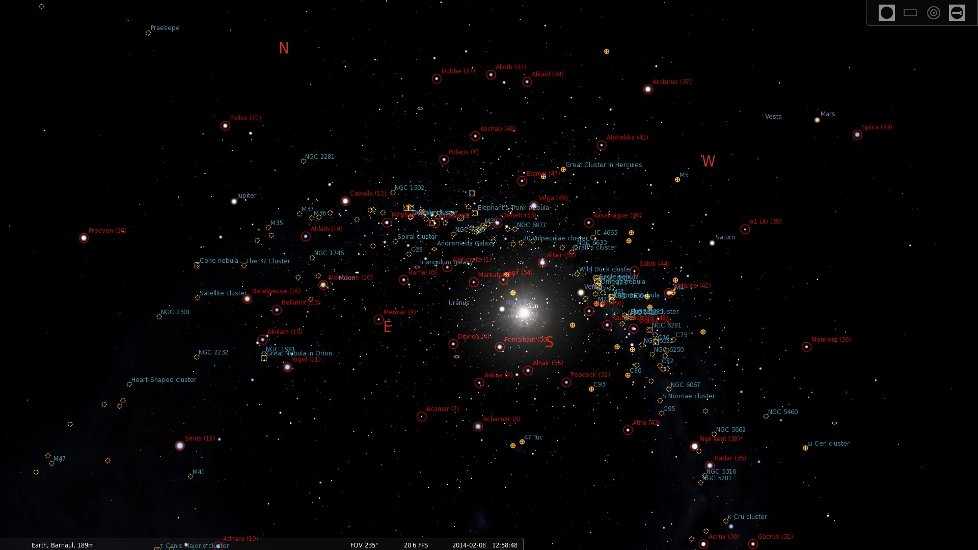
\includegraphics[width=\textwidth]{navstars.jpg}
\label{fig:NavigationalStars}
\caption{Navigational stars on the screen}
\end{figure}

\subsection{Using the Navigational Stars plugin}
\label{sec:plugins:NavigationalStars:using}

\begin{enumerate}
\item Enable the tool by clicking the tool-bar button ``Load at startup''.
\item Click on the Navigational Stars button on the bottom toolbar for displaying markers of navigational stars.
\end{enumerate}


\subsection{Section \big[NavigationalStars\big] in config.ini file}
\label{sec:plugins:NavigationalStars:config}

You can edit \file{config.ini} file by yourself for changes of the
settings for the Navigational Stars plugin -- just make it carefully!

\begin{longtabu} to \textwidth {l|l|X}\toprule
\emph{ID}            & \emph{Type} & \emph{Description}\\\midrule
navstars\_color          & R,G,B & Color of markers of navigational stars  \\\bottomrule
\end{longtabu}

\newpage

\section{Pointer Coordinates Plugin}
\label{sec:plugins:PointerCoordinates}

The Pointer Coordinates plugin shows the coordinates of the mouse pointer.

\begin{figure}[h]
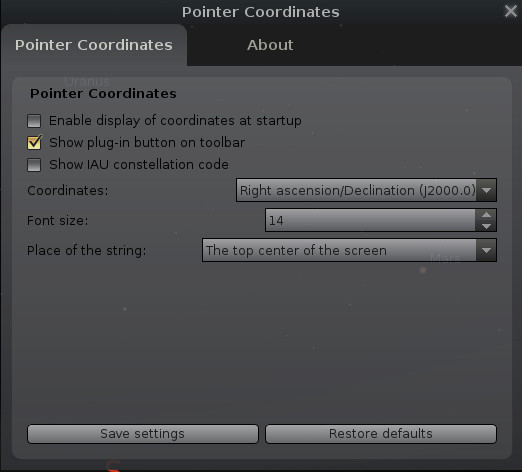
\includegraphics[width=\textwidth]{PointerCoordinates-plugin.jpg}
\label{fig:PointerCoordinates}
\caption{Interface of Pointer Coordinates plugin}
\end{figure}

\subsection{Using the Pointer Coordinates plugin}
\label{sec:plugins:PointerCoordinates:using}

\begin{enumerate}
\item Enable the tool by clicking the tool-bar button ``Load at startup''.
\item Click on the plugin button on the bottom toolbar for displaying the coordinates of the mouse pointer.
\end{enumerate}

\subsection{Section \big[PointerCoordinates\big] in config.ini file}
\label{sec:plugins:PointerCoordinates:config}

You can edit \file{config.ini} file by yourself for changes of the
settings for the Pointer Coordinates plugin -- just make it carefully!

\begin{longtabu} to \textwidth {l|l|X}\toprule
\emph{ID}            & \emph{Type} & \emph{Description}\\\midrule
enable\_at\_startup  & bool & Enable displaying coordinates of the mouse pointer at startup of the plugin\\\midrule
flag\_show\_button   & bool & Enable showing the button of the plugin on bottom toolbar\\\midrule
text\_color          & R,G,B & Color for text with coordinates of the mouse pointer \\\midrule
font\_size           & int & Font size for the displayed coordinates of the mouse pointer \\\midrule
current\_displaying\_place  & string & Specifies the place of displaying coordinates of the mouse pointer. \textit{Possible values}: \keymap{TopRight}, \keymap{TopCenter}, \keymap{RightBottomCorner}, \keymap{Custom}. \textit{Default value}: \keymap{TopRight}. \\\midrule
current\_coordinate\_system & string & Specifies the coordinate system. \textit{Possible values}: \keymap{RaDecJ2000}, \keymap{RaDec}, \keymap{HourAngle}, \keymap{Ecliptic}, \keymap{AltAzi}, \keymap{Galactic}. \textit{Default value}: \keymap{RaDecJ2000}. \\\midrule
custom\_coordinates  & int,int & Specifies the coordinates of the custom place for displaying coordinates of the mouse pointer \\\bottomrule
\end{longtabu}

\newpage

\section{Pulsars Plugin}
\label{sec:plugins:Pulsars}

This plugin plots the position of various pulsars, with object information about each one. Pulsar data is derived from \textit{The ATNF Pulsar Catalogue} (Manchester, R. N., Hobbs, G. B., Teoh, A. \& Hobbs, M., Astron. J., 129, 1993-2006 (2005)\footnote{\url{http://arxiv.org/abs/astro-ph/0412641}}).

\begin{figure}[h]
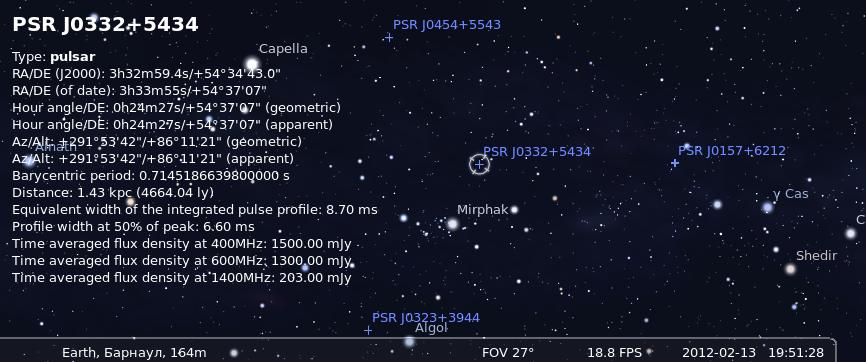
\includegraphics[width=\textwidth]{psr_j0332_5434.jpg}
\label{fig:PSR_J0332-5434}
\caption{PSR J0332-5434}
\end{figure}

\subsection{Using the Pulsars plugin}
\label{sec:plugins:Pulsars:using}

\begin{enumerate}
\item Enable the tool by clicking the tool-bar button ``Load at startup''
\item Find the pulsar by their designation (\emph{PSR J0437-4715} as example)
\end{enumerate}

\subsection{Section \big[Pulsars\big] in config.ini file}
\label{sec:plugins:Pulsars:config}

\begin{longtabu} to \textwidth {l|l|X}\toprule
\emph{ID}               & \emph{Type} & \emph{Description}\\\midrule
last\_update                & string & Date and time of last update\\\midrule
update\_frequency\_days     & int    & Frequency of updates, in days\\\midrule
updates\_enable             & bool   & Enable updates of pulsars catalog from Internet \\\midrule
url                         & string & URL of pulsars catalog \\\midrule
enable\_at\_startup         & bool   & Enable displaying of pulsars at startup of Stellarium \\\midrule
distribution\_enabled       & bool   & Enable distribution mode for the pulsars \\\midrule
flag\_show\_pulsars\_button & bool   & Enable displaying pulsars button on toolbar \\\midrule
marker\_color               & R,G,B  & Color for marker of the pulsars \\\midrule
glitch\_color               & R,G,B  & Color for marker of the pulsars with glitches \\\midrule
use\_separate\_colors       & bool   & Use separate colors for different types of the pulsars \\\bottomrule
\end{longtabu}

\subsection{Format of pulsars catalog}
\label{sec:plugins:Pulsars:format}

To add a new pulsar, open a new line after line 5 and paste the following, note commas and brackets, they are important:

%\newpage

\begin{configfile}
"Pulsar designation":
{
    "RA": "Right ascension (J2000)",
    "DE": "Declination (J2000)",
    "notes": "type of pulsar",
    "distance": value of distance based on electron density 
                model (kpc),
    "period": value of barycentric period of the pulsar (s),
    "parallax": value of annular parallax (mas),
    "bperiod": value of binary period of pulsar (days),
    "pderivative": value of time derivative of barcycentric 
                   period,
    "dmeasure": value of dispersion measure (cm^-3 pc),
    "frequency": value of barycentric rotation frequency (Hz),
    "pfrequency": value of time derivative of barycentric 
                  rotation frequency (s^-2)
    "eccentricity": value of eccentricity,                   
    "w50": value of profile width at 50% of peak (ms),
    "s400": value of time averaged flux density at 
            400 MHz (mJy),
    "s600": value of time averaged flux density at 
            600 MHz (mJy),
    "s1400": value of time averaged flux density at 
             1400 MHz (mJy)    
},

\end{configfile}

%\newpage
\noindent For example, the record for \textbf{PSR J0014+4746} looks like:
\begin{configfile}
"PSR J0014+4746":
{
    "distance": 1.82,
    "dmeasure": 30.85,
    "frequency": 0.805997239145,
    "pfrequency": -3.6669E-16,
    "w50": 88.7,
    "s400": 14,
    "s600": 9,
    "s1400": 3,
    "RA": "00h14m17.75s",
    "DE": "47d46m33.4s"
},
\end{configfile}

\newpage

\section{Text User Interface}
\label{sec:plugins:TextUserInterface}

%\url{http://porpoisehead.net/images/plugin-tui.jpg}

Older versions of Stellarium used to have a little menu system which was
controlled by the cursor keys. This was used primarily by planetarium
system operators to change settings, run scripts and so on. In the
0.10.x series, this function vanished as we totally re-designed the user
interface. This plugin re-implements the ``TUI'', as it was known. Full
list of the commands for the TUI plugin you can read in the section
\href{TUI_Commands}{TUI Commands}.

\subsection{Using the Text User Interface}
\label{sec:plugins:TUI:using}

\begin{enumerate}
\item Activate the text menu using the \key{Alt-T} key.\footnote{This
    used to be hard-coded to \key{M} before version 0.15, but
    \key{Alt-T} runs parallel with \key{Ctrl-T} for switching the GUI
    panels, and frees up \key{M} for the Milky Way. The \key{Alt-T}
    keybinding is hardcoded, i.e., cannot be reconfigured by the
    user.}
\item
  Navigate the menu using the cursors keys.
\item
  To edit a value, press the right cursor until the value you wish to
  change it highlighted with \textgreater{} and \textless{} marks, e.g.\
  \textgreater{}3.142\textless{}. Then press the up and down cursors to
  change the value. You may also type in a new value with the other keys
  on the keyboard.
\end{enumerate}

\subsection{TUI Commands}
\label{sec:plugins:TUI:commands}
\begin{longtabu} to \textwidth {l|l|X}
\toprule
1   & Set Location & (menu group)\\\midrule
1.1 & Latitude & Set the latitude of the observer in degrees\\\midrule
1.2 & Longitude & Set the longitude of the observer in degrees\\\midrule
1.3 & Altitude (m) & Set the altitude of the observer in meters\\\midrule
1.4 & Solar System Body & Select the solar system body on which the observer is\\\midrule
2   & Set Time & (menu group)\\\midrule
2.1 & Sky Time & Set the time and date for which Stellarium will generate the view\\\midrule
2.2 & Set Time Zone & Set the time zone. Zones are split into continent or region, and then by city or province\\\midrule
2.3 & Days keys & The setting ``Calendar'' makes the - = {[} {]} and keys change the date value by calendar days (multiples of 24 hours). 
                  The setting ``Sidereal day'' changes these keys to change the date by sidereal days\\\midrule
2.4 & Preset Sky Time & Select the time which Stellarium starts with (if the ``Sky Time At Start-up'' setting is ``Preset Time''\\\midrule
2.5 & Sky Time At Start-up & The setting ``Actual Time'' sets Stellarium's time to the computer clock when Stellarium runs. 
                             The setting ``Preset Time'' selects a time set in menu item ``Preset Sky Time''\\\midrule
2.6 & Time Display Format & Change how Stellarium formats time values. ``system default'' takes the format from the computer settings, 
                            or it is possible to select 24 hour or 12 hour clock modes\\\midrule
2.7 & Date Display Format & Change how Stellarium formats date values. ``system default'' takes the format from the computer settings, 
                            or it is possible to select ``yyyymmdd'', ``ddmmyyyy'' or ``mmddyyyy'' modes\\\midrule
3    & General & (menu group)\\\midrule
3.1  & Sky Culture  & Select the sky culture to use (changes constellation lines, names, artwork)\\\midrule
3.2  & Sky Language & Change the language used to describe objects in the sky\\\midrule
4    & Stars & (menu group)\\\midrule
4.1  & Show & Turn on/off star rendering\\\midrule
4.2  & Star Magnitude Multiplier & Can be used to change the brightness of the stars which are visible at a given zoom level. 
                                   This may be used to simulate local seeing conditions - the lower the value, the less stars will be visible\\\midrule
4.3  & Maximum Magnitude to Label & Changes how many stars get labelled according to their apparent magnitude (if star labels are turned on)\\\midrule
4.4  & Twinkling & Sets how strong the star twinkling effect is - zero is off, the higher the value the more the stars will twinkle.\\\midrule
5    & Colors & (menu group)\\\midrule
5.1  & Constellation Lines         & Changes the colour of the constellation lines\\\midrule
5.2  & Constellation Names         & Changes the colour of the labels used to name stars\\\midrule
5.3  & Constellation Art Intensity & Changes the brightness of the constellation artconstellation art\\\midrule
5.4  & Constellation Boundaries    & Changes the colour of the constellation boundary lines\\\midrule
5.5  & Cardinal Points & Changes the colour of the cardinal points markers\\\midrule
5.6  & Planet Names    & Changes the colour of the labels for planets\\\midrule
5.7  & Planet Orbits   & Changes the colour of the orbital guide lines for planets\\\midrule
5.8  & Planet Trails   & Changes the colour of the planet trails lines\\\midrule
5.9  & Meridian Line   & Changes the colour of the meridian line\\\midrule
5.10 & Azimuthal Grid  & Changes the colour of the lines and labels for the azimuthal grid\\\midrule
5.11 & Equatorial Grid & Changes the colour of the lines and labels for the equatorial grid\\\midrule
5.12 & Equator Line    & Changes the colour of the equator line\\\midrule
5.13 & Ecliptic Line   & Changes the colour of the ecliptic line\\\midrule
5.14 & Nebula Names    & Changes the colour of the labels for nebulae\\\midrule
5.15 & Nebula Circles  & Changes the colour of the circles used to denote the positions of nebulae (only when enabled int he configuration file, note this feature is off by default)\\\midrule
6   & Effects & (menu group)\\\midrule
6.1 & Light Pollution Luminance & Changes the intensity of the light pollution simulation\\\midrule
6.2 & Landscape & Used to select the landscape which Stellarium draws when ground drawing is enabled\\\midrule
6.3 & Manual zoom & Changes the behaviour of the \key{/} and \key{\textbackslash{}} keys. When set to ``No'', these keys zoom all the way to a level defined
by object type (auto zoom mode). When set to ``Yes'', these keys zoom in and out a smaller amount and multiple presses are required\\\midrule
6.4 & Object Sizing Rule & When set to ``Magnitude'', stars are drawn with a size based on their apparent magnitude. When set to ``Point'' all stars are drawn with the same size on the screen\\\midrule
6.5 & Magnitude Sizing Multiplier & Changes the size of the stars when ``Object Sizing Rule'' is set to ``Magnitude''\\\midrule
6.6 & Milky Way intensity & Changes the brightness of the Milky Way texture\\\midrule
6.7 & Maximum Nebula Magnitude to Label & Changes the magnitude limit for labelling of nebulae\\\midrule
6.8 & Zoom Duration & Sets the time for zoom operations to take (in seconds)\\\midrule
6.9 & Cursor Timeout & Sets the number of seconds of mouse inactivity before the cursor vanishes\\\midrule
6.10 & Setting Landscape Sets Location & If ``Yes'' then changing the landscape will move the observer location to the location for that landscape (if one is known). 
                                         Setting this to ``No'' means the observer location is not modified when the landscape is changed.\\\midrule
7 & Scripts & (menu group)\\\midrule
7.1 & Local Script & Run a script from the scripts sub-directory of the User Directory or Installation Directory (see section~\ref{sec:FilesAndDirectories} (Files and Directories))\\\midrule
7.2 & CD/DVD Script          & Run a script from a CD or DVD (only used in planetarium set-ups)\\\midrule
8   & Administration         & (menu group)\\\midrule
8.1 & Load Default Configuration & Reset all settings according to the main configuration file\\\midrule
8.2 & Save Current Configuration as Default & Save the current settings to the main configuration file\\\midrule
8.3 & Shutdown               & Quit Stellarium\\\midrule
8.4 & Update me via Internet & Only used in planetarium set-ups\\\midrule
8.5 & Set UI Locale          & Change the language used for the user interface\\\bottomrule
\end{longtabu}




%%% Local Variables: 
%%% mode: latex
%%% TeX-master: "guide"
%%% End: 

